\documentclass[10pt]{article}
\usepackage[utf8]{inputenc}
\usepackage{graphicx}
\usepackage{caption}
\usepackage{subcaption}
\usepackage{booktabs}
\usepackage[margin=0.5in]{geometry} % Set all margins to 1 inch



\begin{document}

% \title{TP 3}
% \author{Mahdi Moghadasi \\ 20184188 \and Ibrahim Ould Saada \\ 20151421}
% \date{}
% \maketitle
\noindent \textbf{TP 3} \hfill \textbf{Mahdi Moghadasi (20184188), Ibrahim Ould Saada (20151421)}


\section{Visualisation des Métriques et Calcul des Informations Pertinentes}

\begin{figure}[h]
\centering
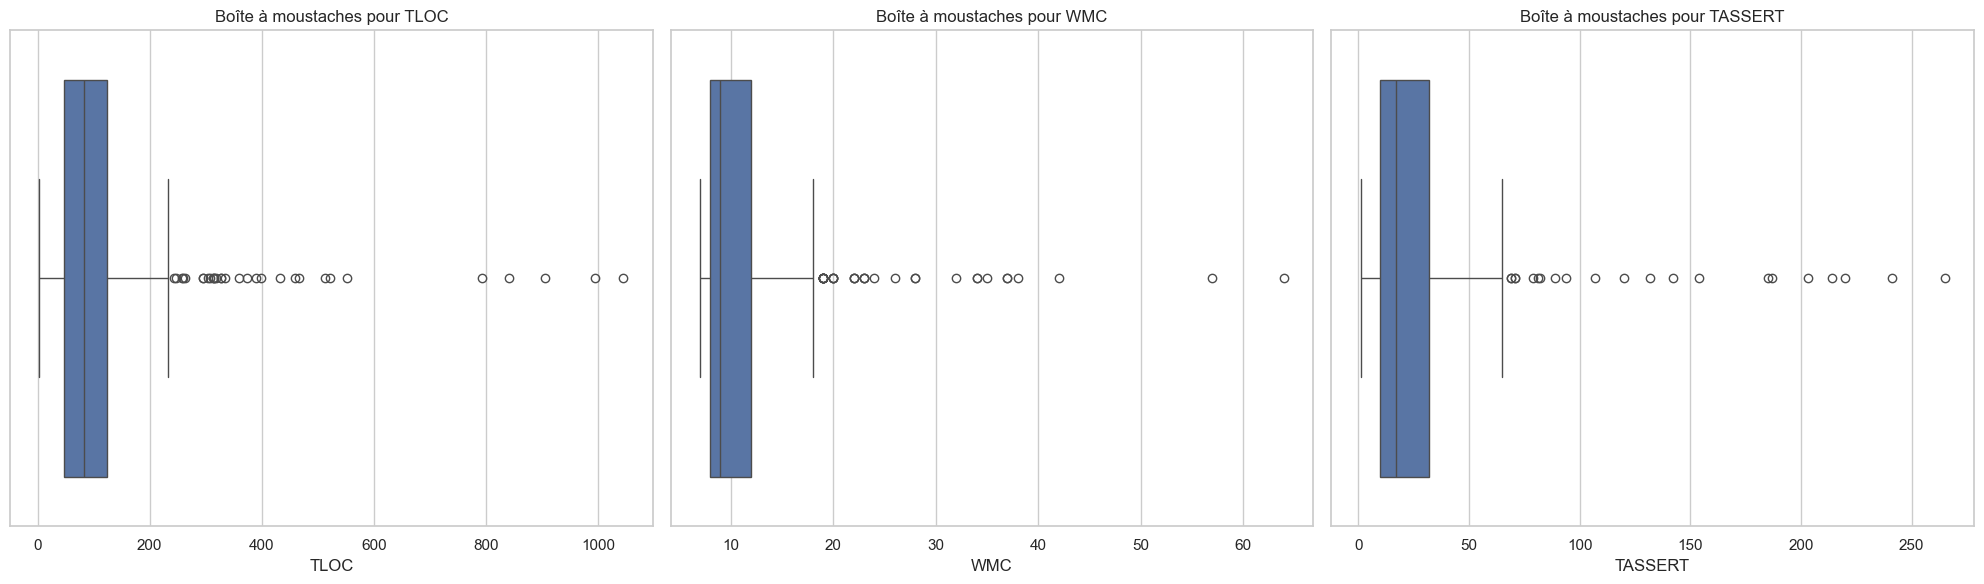
\includegraphics[width=1\textwidth]{boxplot.png}
\caption{Boxplot des métriques}
\end{figure}

Voici un résumé des statistiques descriptives pour les trois métriques :

\begin{table}[h]
\centering
\resizebox{\textwidth}{!}{%
    \begin{tabular}{|l|c|c|c|c|c|c|c|c|c|c|c|}
    \hline
    Métrique & Nombre d'observations & Moyenne & Écart-type & Minimum & l & m & u & Maximum & s & i & d \\ \hline
    TLOC & 351 & 115.13 & 130.87 & 3 & 47.5 & 83 & 124.5 & 1045 & 240 & 0 (-68) & 77 \\ \hline
    WMC & 351 & 11.58 & 6.53 & 7 & 8 & 9 & 12 & 64 & 18 & 2 & 4 \\ \hline
    TASSERT & 351 & 27.19 & 34.80 & 1 & 10 & 17 & 32 & 265 & 65 & 0 (-23) & 22 \\ \hline
    \end{tabular}
    }
\caption{Résumé des statistiques descriptives}
\end{table}

\begin{figure}[h]
\centering
\begin{subfigure}{.31\textwidth}
  \centering
  \includegraphics[width=\linewidth]{Histogram-TLOC.png}
  \caption{Histogramme de TLOC}
\end{subfigure}%
\hfill
\begin{subfigure}{.31\textwidth}
  \centering
  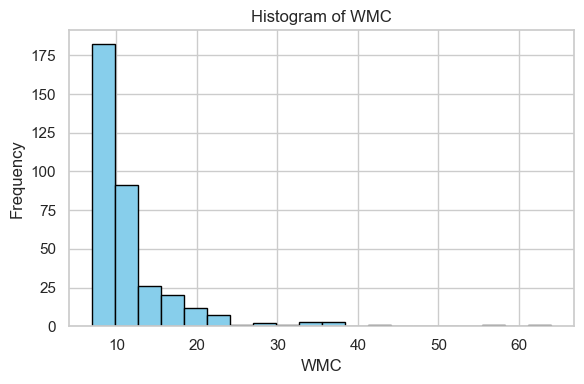
\includegraphics[width=\linewidth]{Histogram-WMC.png}
  \caption{Histogramme de WMC}
\end{subfigure}%
\hfill
\begin{subfigure}{.31\textwidth}
  \centering
  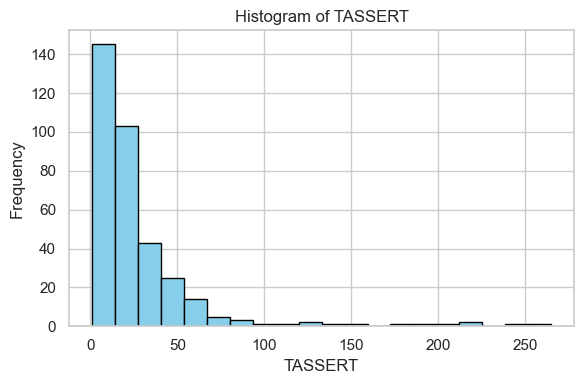
\includegraphics[width=\linewidth]{Histogram-Tassert.png}
  \caption{Histogramme de TASSERT}
\end{subfigure}
\caption{Histogrammes des métriques}
\end{figure}

\subsection*{Interprétation des distributions:}

Les trois métriques (TLOC, WMC, TASSERT) démontrent des distributions inclinées vers la droite(Histogram ou boite à moustache) .Les grands écarts-types pour chaque métrique reflètent la variabilité considérable dans nos données.

\subsubsection{TLOC (Total Lines of Code)}

La distribution de TLOC est fortement inclinée vers la droite. Cela est évident à partir de la boite à moustache et confirmé par les statistiques descriptives. La plupart des classes ont relativement peu de lignes de code, mais il y a des cas atypiques avec des valeurs considérablement plus élevées. La médiane, à 83 lignes, est la meilleure mesure de la tendance centrale ici( par rapport a la moyenne), indiquant que la moitié des classes ont moins de 83 lignes de code. Un grand écart-type d'environ 131 lignes suggère une large variabilité dans la taille des classes. Selon la boite a moustache, nous avons beaucoup de classes atypiques avec des valeurs de TLOC très élevées; Surtout entre la limite supérieure et un peu près de 600.

\subsubsection{WMC (Weighted Methods per Class)}

Comme le TLOC, il est incliné vers la droite.  indiquant que la plupart des classes ont moins de méthodes. La moyenne d'environ 11,6 méthodes par classe est influencée par des classes avec de nombreuses méthodes. La médiane est de 9 méthodes, suggérant que plus de la moitié des classes sont relativement simples. Un écart-type modéré de 6,53 indique une variabilité, mais pas aussi prononcée que dans le TLOC. La moustache supérieure va jusqu'à 18 méthodes. Nous voyons quelques classes atypiques(avec plus de 18 méthodes) surtout entre la limite supérieure (18) et un peu près de 40.

\subsubsection{TASSERT (Total Assertions)}

TASSERT est également incliné vers la droite, montrant que bien que la plupart des classes aient moins d'assertions, certaines en ont un grand nombre. La médiane de 17 assertions montre plus précisément le nombre d'assertions typique d'une classe(par rapport a la moyenne). Un très grand écart-type de 34,8 indique une variabilité dans le nombre d'assertions entre les classes. La moustache supérieure de la boîte à moustaches s'étendant jusqu'à 65 assertions suggère que les classes au-delà de ce nombre ont un comptes d'assertions très élevés.
% La moyenne d'environ 27,2 assertions est faussée par des classes avec un très grand nombre d'assertions.




\section{Étude des Corrélations et Calcul des Droites de Régression}


\subsection{Avec tous les points}
\begin{figure}[h]
\centering
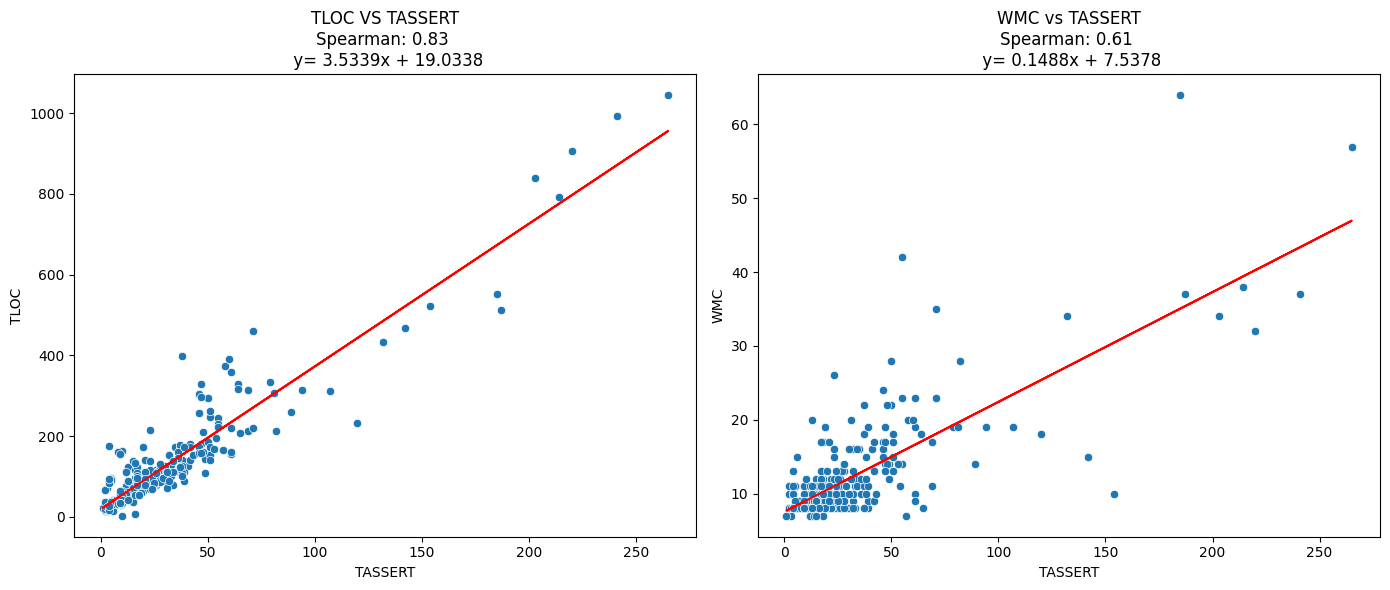
\includegraphics[width=0.7\textwidth]{correlations.png}
\caption{Corrélations et régression entre les métriques}
\end{figure}

Les trois métriques ne sont pas normales. Alors on a utilisé le coefficient de corrélation Spearman pour cette analyse.

\subsubsection{TLOC et TASSERT}
\begin{itemize}
    \item \textbf{Coefficient de Spearman} : 0.83. Cela indique une forte corrélation positive entre TASSERT et TLOC. Plus le nombre d'assertions de test (TASSERT) est élevé, plus le nombre total de lignes de code de test (TLOC) tend à être élevé.
    \item \textbf{Équation de régression} : \( y = 3.53x + 19.03 \) 
    \begin{itemize}
        \item \textbf{Pente (3.53)} : Pour chaque augmentation d'une unité de TASSERT, TLOC augmente en moyenne de 3.53 unités.
        \item \textbf{Ordonnée à l'origine (19.03)} : Lorsque TASSERT est 0, la valeur estimée de TLOC est d'environ 19.03.. Cela pourrait indiquer un nombre de base de lignes de code de test présentes indépendamment du nombre d'assertions.
    \end{itemize}
\end{itemize}

\subsubsection{WMC ET TASSERT}
\begin{itemize}
    \item \textbf{Coefficient de Spearman} : 0.61. Cela indique une corrélation positive modérée entre TASSERT et WMC. Cela suggère que, dans une certaine mesure, à mesure que le nombre d'assertions augmente, la complexité des méthodes par classe (WMC) augmente également.
    \item \textbf{Équation de régression} : \( y = 0.15x + 7.54 \)
    \begin{itemize}
        \item \textbf{Pente (0.15)} : Une augmentation d'une unité de TASSERT est associée à une augmentation moyenne de 0.15 unité de WMC.
        \item \textbf{Ordonnée à l'origine (7.54)} : Si TASSERT est 0, la valeur estimée de WMC est d'environ 7.54. Cela peut suggérer un niveau de base de complexité des méthodes dans les classes analysées, indépendant du nombre d'assertions.
    \end{itemize}
\end{itemize}

\subsection{En excluant les points extrêmes}

\begin{figure}[h]
\centering
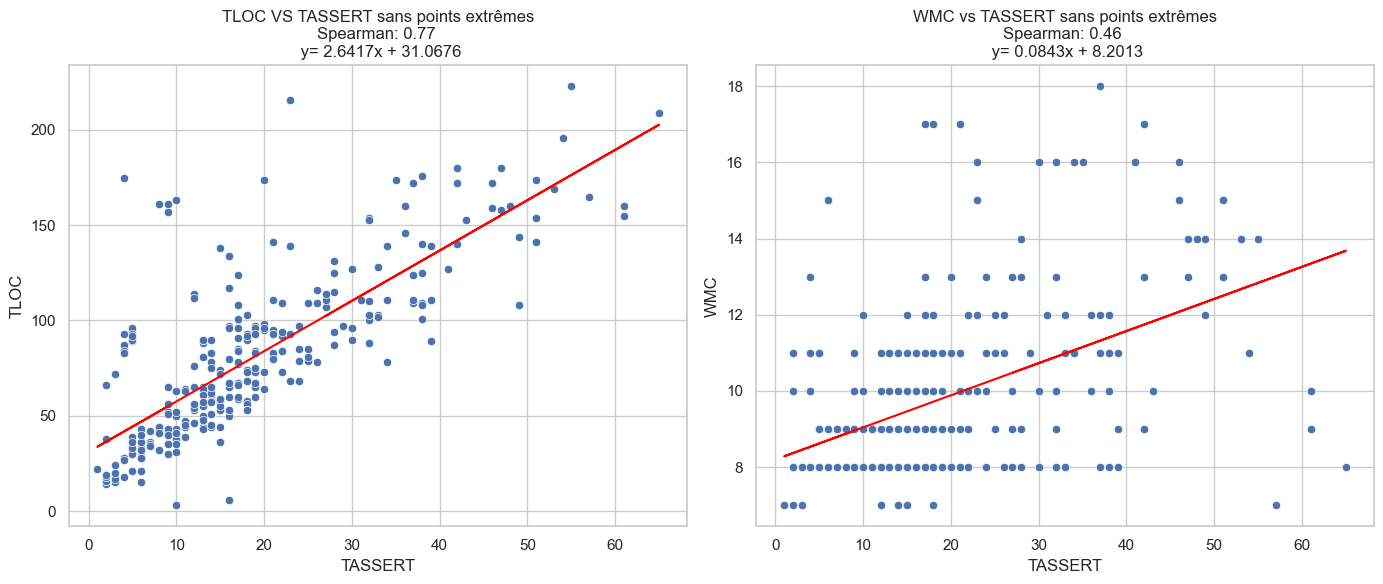
\includegraphics[width=0.7\textwidth]{correlations-no-outliers.png}
\caption{Corrélations et régression entre les métriques sans les points extrêmes}
\end{figure}

Nous voyons que le coefficient de spearman et la pente de la droite de régression se réduisent un peu mais dans les deux cas, on peut dire que l'interprétation reste la même. On a toujours une forte corrélations positive pour le cas TLOC vs TASSERT et une corrélations positive modérée pour le cas WMC vs TASSERT, ce qui est attendu dans notre cas parce que le coefficient spearman n'est pas autant affecté par les points extrêmes que pearson.

\subsection{Conclusion}
Les résultats indiquent des relations positives entre TASSERT et les deux autres mesures (TLOC et WMC), étant plus forte avec TLOC. 


\section{Évaluation de l'Hypothèse sur la Complexité des Classes}

\subsection{Choix d'Étude}

\begin{itemize}
    \item\textbf{Quasi-Expérience :} Analyser les données des classes de tests du projet JFreechart pour comparer la complexité des classes avec plus de 20 assertions par rapport à celles avec moins de 20 assertions.
\end{itemize}

\subsection{Énoncé des Hypothèses}

\begin{itemize}
    \item \textbf{Hypothèse nulle (H0):} Il n'y a pas de différence significative de complexité entre les classes avec plus de 20 assertions et celles avec moins.
    \item\textbf{Hypothèse alternative (H1) :} Les classes avec plus de 20 assertions sont plus complexes.
\end{itemize}


\subsection{Définition des Variables}
\begin{itemize}
    \item\textbf{Variable indépendante :} Le nombre d'assertions dans une classe (pour séparer en deux groupes : $> 20$ , $\leq20$).
    \item\textbf{Variables dépendantes :}  Les métriques TLOC et WMC.
\end{itemize}


\subsection{ interprétation et généralisation des résultats}

\subsubsection{Méthodologie}
Pour tester nos hypothèses, nous avons pris les 2 variables TLOC et WMC en compte. d'abord, nous faisons le test Shapiro-Wilk pour tester la normalité de 2 différents groupes \textit{( assertion plus de 20 et moins ou égal à 20) }  pour les deux métriques. après, en considerant le résultat de Shapiro-Wilk, nous avons décidé de faire le test de Mann-Whitney pour les deux métriques et analyser les résultats.

\subsubsection{Test Shapiro-Wilk}

\noindent
\begin{minipage}[t]{0.5\textwidth}
\vspace{0pt}
Les résultats du test indiquent des p-value proche de zéro et significativement inférieures au seuil de 0.05 pour toutes les distributions testée. Nous rejetons l'hypothèse nulle de ce teste (normalité de la population) et concluons que les données ne suivent pas une distribution normale. Cela justifie l'utilisation de test Mann-Whitney pour comparer les groupes.
\end{minipage}
\hfill
\begin{minipage}[t]{0.45\textwidth}
\vspace{0pt}
\begin{tabular}{|l|l|l|}
\hline
\textbf{Test} & \textbf{Statistic} & \textbf{p-value} \\ \hline
TLOC $\leq20$ & 0.9323 & \( 1.94 \times 10^{-8} \) \\ \hline
TLOC $>20$ & 0.6583 & \( 2.74 \times 10^{-16} \) \\ \hline
WMC $\leq20$ & 0.7033 & \( 2.56 \times 10^{-19} \) \\ \hline
WMC $>20$ & 0.7292 & \( 1.78 \times 10^{-14} \) \\ \hline
\end{tabular}
\captionof{table}{Shapiro-Wilk Test Results}
\label{tab:shapiro_results}
\end{minipage}


\subsubsection{Test U de Mann-Whitney }
Le test de Mann-Whitney a été utilisé pour comparer les distributions de \textit{TLOC} et \textit{WMC} entre les classes avec plus de 20 assertions et celles avec 20 assertions ou moins. Ce teste considère les rangs et donc la médiane de deux groupes. Selon la direction Spécifique de l'hypothèse ( l'augmentation de la complexité des classes avec plus de 20 assertions) , nous avons fait un test à droite(unilatéral). Les p-values obtenues sont extrêmement faibles et inferieurs a notre seuil de 0.05. Ces résultats indiquent une différence statistiquement significative entre les deux groupes pour les deux mesures de complexité, soutenant l'hypothèse alternative dans les deux cas indiquant que les classes avec plus de 20 assertions sont plus complexes que celles avec moins de 20 assertions.

\begin{table}[h]
\centering
\begin{tabular}{|l|l|l|}
\hline
\textbf{Measure} & \textbf{Statistic} & \textbf{p-value} \\ \hline
TLOC & 27392.5 & \( 6.02 \times 10^{-44} \) \\ \hline
WMC & 24199.0 & \( 8.89 \times 10^{-27} \) \\ \hline
\end{tabular}
\caption{Résultats du test de Mann-Whitney U}
\label{tab:mann_whitney_results}
\end{table}

% \noindent
% \begin{minipage}[t]{0.5\textwidth}
% \vspace{0pt}
% Le test de Mann-Whitney a été utilisé pour comparer les distributions de \textit{TLOC} et \textit{WMC} entre les classes avec plus de 20 assertions et celles avec 20 assertions ou moins. Ce teste considère les rangs et donc la médiane de deux groupes. Selon la direction Spécifique de l'hypothèse ( l'augmentation de la complexité des classes avec plus de 20 assertions) , nous avons fait un test à droite(unilatéral). Les p-values obtenues sont extrêmement faibles et inferieurs a notre seuil de 0.05. Ces résultats indiquent une différence statistiquement significative entre les deux groupes pour les deux mesures de complexité, soutenant l'hypothèse alternative dans les deux cas indiquant que les classes avec plus de 20 assertions sont plus complexes que celles avec moins de 20 assertions.
% \end{minipage}
% \hfill
% \begin{minipage}[t]{0.45\textwidth}
% \vspace{0pt}
% \begin{tabular}{|l|l|l|}
% \hline
% \textbf{Measure} & \textbf{Statistic} & \textbf{p-value} \\ \hline
% TLOC & 27392.5 & \( 6.02 \times 10^{-44} \) \\ \hline
% WMC & 24199.0 & \( 8.89 \times 10^{-27} \) \\ \hline
% \end{tabular}
% \captionof{table}{Résultats du test de Mann-Whitney U}
% \label{tab:mann_whitney_results}
% \end{minipage}





\subsection{Discussion des Menaces à la Validité}


\subsubsection{Validité Interne}
Pour la validité interne, Bien que nous ayons utilisé TLOC et WMC comme indicateurs de la complexité, ces mesures pourraient ne pas capturer tous les aspects de la complexité des classes et il est difficile de  dire avec les informations que nous avons si les changement dans la complexité (TLOC et WMC) sont attribuable aux changement dans le nombre d'assertion(Tassert).

\subsubsection{Validité Externe}
En ce qui concerne la validité externe, notre étude est limitée par sa focalisation sur le projet JFreechart. Bien que cela fournisse un contexte spécifique et détaillé pour notre analyse, cela peut également limiter la généralisabilité de nos conclusions à d'autres projets ou environnements de développement logiciel.

\subsubsection{Validité de Construction}
La validité de construction dans notre étude est également un point important. Les métriques que nous avons utilisés sont appropriés pour les données que nous avons analysées. Cependant,l'utilisation d'autres métriques pourrait offrir un point de vue différent. La définition de ce que signifie être "plus complexe" dans le contexte de la programmation, doit être clairement défini pour éviter toute ambiguïté.

\subsubsection{Validité de Conclusion}
Enfin, pour ce qui est de la validité de conclusion, Nous avons déjà toutes les menaces de la validité interne.De plus, bien que nous ayons trouvé une différence statistiquement significative, le choix du seuil de p-value, généralement fixé à 0.05, joue un rôle important dans la possibilité d'avoir un faux positifs. Ce choix doit être justifié pour renforcer la fiabilité de nos conclusions.


\end{document}  
